\documentclass[12pt,a4paper,openright,twoside]{book}
\usepackage[utf8]{inputenc}
\usepackage{disi-thesis}
\usepackage{code-lstlistings}
\usepackage{notes}
\usepackage{shortcuts}
\usepackage{acronym}
\usepackage{amsmath}
\usepackage{mathtools}

\school{\unibo}
\programme{Corso di Laurea
%[Magistrale?]
in Ingegneria e Scienze Informatiche}
\title{
%Fancy Title
Studio e applicazione del filtro di Kalman e sue varianti per il tracciamento di corpi celesti
}
\author{
%Candidate Name
Marco Buda
}
\date{\today}
\subject{
%Supervisor's course name
Metodi Numerici
}
\supervisor{Prof.ssa
%Supervisor Here
Damiana Lazzaro
}
%\cosupervisor{Dott. CoSupervisor 1}
%\morecosupervisor{Dott. CoSupervisor 2}
\session{
%I
II % TODO: verificare
}
\academicyear{
%2022-2023
2024-2025
}

% Definition of acronyms
\acrodef{IoT}{Internet of Thing}
\acrodef{vm}[VM]{Virtual Machine}


\mainlinespacing{1.241} % line spacing in mainmatter, comment to default (1)

\lstset{language=Python,basicstyle=\small\ttfamily}

\begin{document}

\frontmatter\frontispiece

\begin{abstract}	
% Max 2000 characters, strict.
TODO
\end{abstract}

\iffalse
\begin{dedication} % this is optional
Optional. Max a few lines.
\end{dedication}
\fi

%----------------------------------------------------------------------------------------
\tableofcontents   
\listoffigures     % (optional) comment if empty
\lstlistoflistings % (optional) comment if empty
%----------------------------------------------------------------------------------------

\mainmatter

%----------------------------------------------------------------------------------------
\chapter{Introduzione}
\label{chap:introduction}
%----------------------------------------------------------------------------------------

TODO

\iffalse
Write your intro here.
\sidenote{Add sidenotes in this way. They are named after the author of the thesis}

You can use acronyms that your defined previously,
such as \ac{IoT}.
%
If you use acronyms twice,
they will be written in full only once
(indeed, you can mention the \ac{IoT} now without it being fully explained).
%
In some cases, you may need a plural form of the acronym.
%
For instance,
that you are discussing \acp{vm},
you may need both \ac{vm} and \acp{vm}.
\fi

\paragraph{Struttura della tesi}

TODO

% \note{At the end, describe the structure of the paper}

%----------------------------------------------------------------------------------------
\chapter{Fondamenti teorici}
%----------------------------------------------------------------------------------------

In questo capitolo si definiscono i concetti di base su cui si svilupperanno gli argomenti di questa tesi, insieme ai modelli matematici che li descrivono. Si presenta, inoltre, una costruzione algebrica del filtro di Kalman e si offre una panoramica delle sue varianti.

\section{I sistemi dinamici}

Un sistema dinamico è un qualunque sistema che evolve nel tempo secondo una determinata legge. \\

A seconda dell'obiettivo, si individuano le proprietà del sistema che interessa esaminare (es.: posizione e velocità di un oggetto), dette variabili di stato, e le si raccoglie in un vettore, generalmente $x\in\mathbb{R}^n$, andando a definire una cosiddetta rappresentazione in spazio di stato. \\
Nella forma generale, si considera il tempo come continuo ($t\in\mathbb{R}$), per cui si parla di modelli continui, espressi con equazioni differenziali:
$$\dfrac{d}{dt}\bigl(x(t)\bigr)=f\bigl(t,x(t)\bigr)$$ \pagebreak

Tuttavia, si può decidere di considerare lo stato soltanto in determinati istanti $t_k$. Ne risultano modelli discreti, su cui si concentrerà questa tesi, i quali possono essere espressi con relazioni di ricorrenza:
$$x_k=f(k,x_{k-1})$$

In genere si sceglie di esplicitare la presenza di ingressi $u\in\mathbb{R}^l$ nel sistema (\textit{control input}, es.: forza di gravità, propulsione...), assunti deterministici, e di misurazioni $z\in\mathbb{R}^m$ (\textit{measurement}), effettuate sulle variabili osservate. \\
Dunque il modello viene espresso con le equazioni:
\begin{gather*}
x_k=f(k,x_{k-1},u_{k-1}) \\
z_k=h(k,x_k)
\end{gather*}
La prima è detta ``equazione di stato'' e la seconda ``trasformazione di uscita''. \\

Modellizzare la realtà comporta spesso che non si conosca la vera legge di evoluzione $f_\text{reale}$, ma solo una sua approssimazione, quindi soggetta a disturbi o imprecisioni (\textit{process noise}, $w\in\mathbb{R}^n$), da cui l'importanza di effettuare misurazioni periodiche per monitorare la reale evoluzione dello stato.

Poiché le misurazioni stesse sono soggette a disturbi (\textit{measurement noise}, $v\in\mathbb{R}^m$), il modello completo diventa:
\begin{gather}
x_k=f(k,x_{k-1},u_{k-1})+w_{k-1}\label{eq:fdet} \\
z_k=h(k,x_k)+v_k\label{eq:hdet}
\end{gather}

Un caso particolare riguarda i modelli lineari, cioè esprimibili nella seguente forma matriciale:
\begin{gather}
x_k=A_kx_{k-1}+B_ku_{k-1}+w_{k-1} \label{eq:transition}\\
z_k=H_kx_k+v_k \label{eq:output}
\end{gather}
In questo caso, $A_k\in\mathbb{R}^{n\times n}$ è detta ``matrice dinamica'' e determina l'evoluzione dello stato dal passo $k-1$ al passo $k$ in assenza di ingressi e disturbi, $B_k\in\mathbb{R}^{l\times n}$ è detta ``matrice di ingresso'' e determina il contributo degli ingressi che agiscono dal passo $k-1$ al passo $k$ e $H_k\in\mathbb{R}^{m\times n}$ è detta ``matrice di uscita'' e determina le variabili osservate in base alle variabili da stimare. \\

In generale, i modelli sono tempo-varianti (o non stazionari), da cui $k$ al pedice di $A_k$, $B_k$ e $H_k$, ma si evidenziano i modelli LTI, ossia lineari tempo-invarianti (o lineari stazionari) in cui le matrici $A$, $B$ e $H$ sono costanti nel tempo. \\

Dalla combinazione delle imprecisioni nel modello e nelle misurazioni, nasce la necessità di algoritmi che raccolgano ed interpretino i dati osservati per determinare una stima (\textit{state estimate}, $\hat{x}$) dello stato reale (\textit{ground truth}, $x$). Questi algoritmi sono detti, appunto, stimatori.

\section{Il filtro di Kalman}

Il filtro di Kalman~\cite{10.1115/1.3662552}~\cite{WelchB95}~\cite{10.1145/3363294} è uno stimatore lineare ricorsivo che minimizza l'errore quadratico medio. \\
L'aspetto ricorsivo implica, innanzitutto, che si tratta di un filtro a tempo discreto e si rifà al fatto che ogni stima $\hat{x}_k$ è determinata in base alla stima precedente $\hat{x}_{k-1}$ e alla misurazione attuale $z_k$, senza richiedere l'utilizzo esplicito di $\hat{x}_0,\hat{x}_1,...,\hat{x}_{k-2}$ o $z_1,...,z_{k-1}$. Si tratta di uno dei principali vantaggi del filtro, in quanto riduce sia la complessità temporale che quella spaziale, senza compromettere l'ottimalità. \\
Come anticipato, l'ottimalità è definita dal fatto che, ad ogni passo $k$, l'algoritmo produce la stima $\hat{x}_k$ che minimizza la quantità $\mathbb{E}[\lVert e_k\rVert^2]$, con $e_k=\hat{x}_k-x_k$. \\

Il filtro è applicabile a un qualsiasi modello lineare a tempo discreto, anche tempo-variante, ossia descritto dalle equazioni \ref{eq:transition} e \ref{eq:output}.

Sono posti, però, vincoli di non correlazione sulle variabili aleatorie:
\begin{align*}
& \mathrm{Cov}(w_k,v_j)=0_{n\times m}, && \forall\,k,\forall\,j \\
& \mathrm{Cov}(w_k,u_j)=0_{n\times l}, && \forall\,k,\forall\,0\leq j\leq k-1 \\
& \mathrm{Cov}(v_k,u_j)=0_{m\times l}, && \forall\,k,\forall\,0\leq j\leq k-2 \\
& \mathrm{Cov}(w_k,w_j)=0_{n\times n}, && \forall\,k,\forall\,j\neq k \\
& \mathrm{Cov}(v_k,v_j)=0_{m\times m}, && \forall\,k,\forall\,j\neq k \\
& \mathrm{Cov}(w_k,x_0)=0_{n\times n}, && \forall\,k \\
& \mathrm{Cov}(v_k,x_0)=0_{m\times n}, && \forall\,k
\end{align*}

Infine, nelle formulazioni standard del filtro, si richiede che $w$ e $v$ siano privi di \textit{bias}, ossia che $\mathbb{E}[w_k]=\underline{0}$ e $\mathbb{E}[v_k]=\underline{0}$, ad ogni passo $k$.

\section{Costruzione del filtro lineare}

Nella letteratura sono riportate diverse derivazioni e dimostrazioni di ottimalità del filtro di Kalman~\cite[pp.~107-113]{10.5555/2823801}~\cite{10.48550/arXiv.1910.03558}. Si presenta qui una costruzione algebrica il più elementare possibile. \\

Il primo passo è descrivere l'espressione che calcoli la stima $\hat{x}_k$. Al passo $k\geq 1$ sono disponibili le informazioni riguardo $\hat{x}_{k-1}$, $u_{k-1}$ e $z_k$, per cui l'espressione lineare avrà la forma generica:
\begin{equation} \label{eq:generic-estimate}
\hat{x}_k=\mathcal{A}_k\hat{x}_{k-1}+\mathcal{B}_ku_{k-1}+\mathcal{K}_kz_k
\end{equation}
Per quanto riguarda il passo $k=0$, la scelta della stima iniziale $\hat{x}_0$ è libera, purché sia deterministica. Se si hanno informazioni sulla distribuzione di $x_0$, è consigliabile scegliere $\hat{x}_0=\mathbb{E}[x_0]$. \\

Una condizione implicita sul filtro richiede che anche l'errore sulle stime generate $e_k$ sia privo di \textit{bias}, ossia, ad ogni passo $k$:
$$\mathbb{E}[e_k]=\mathbb{E}[\hat{x}_k-x_k]=\underline{0}$$
Da questa condizione si otterranno informazioni sulle matrici incognite $\mathcal{A}$, $\mathcal{B}$ e $\mathcal{K}$. In effetti, considerando per $k\geq 1$ e sostituendo $\hat{x}_k$ con la sua definizione (eq.~\ref{eq:generic-estimate}), si ottiene:
$$\mathbb{E}[\mathcal{A}_k\hat{x}_{k-1}+\mathcal{B}_ku_{k-1}+\mathcal{K}_kz_k-x_k]=\underline{0}$$
Successivamente, sostituendo $z_k$ con la sua definizione (eq.~\ref{eq:output}):
$$\mathbb{E}\left[\mathcal{A}_k\hat{x}_{k-1}+\mathcal{B}_ku_{k-1}+\mathcal{K}_k\bigl(H_kx_k+v_k\bigr)-x_k\right]=\underline{0}$$
Sostituendo $x_k$ con la relazione di ricorrenza (eq.~\ref{eq:transition}) e manipolando i termini:
\begin{gather*}
\begin{multlined}[\textwidth]
\mathbb{E}\Bigl[\mathcal{A}_k\hat{x}_{k-1}+\mathcal{B}_ku_{k-1}+\mathcal{K}_k\Bigl(H_k\bigl(A_kx_{k-1}+B_ku_{k-1}+w_{k-1}\bigr)+v_k\Bigr)+ \\
-\bigl(A_kx_{k-1}+B_ku_{k-1}+w_{k-1}\bigr)\Bigr]=\underline{0}
\end{multlined} \\
\begin{multlined}[\textwidth]
\Rightarrow\mathbb{E}\bigl[\mathcal{A}_k\hat{x}_{k-1}+\mathcal{B}_ku_{k-1}+\mathcal{K}_kH_kA_kx_{k-1}+\mathcal{K}_kH_kB_ku_{k-1}+\mathcal{K}_kH_kw_{k-1}+ \\
+\mathcal{K}_kv_k-A_kx_{k-1}-B_ku_{k-1}-w_{k-1}\bigr]=\underline{0}
\end{multlined} \\
\begin{multlined}[\textwidth]
\Rightarrow\mathbb{E}\bigl[\mathcal{A}_k\hat{x}_{k-1}+\mathcal{B}_ku_{k-1}+\mathcal{K}_kH_kA_kx_{k-1}+\mathcal{K}_kH_kB_ku_{k-1}+\mathcal{K}_kH_kw_{k-1}+ \\
+\mathcal{K}_kv_k-A_kx_{k-1}-B_ku_{k-1}-w_{k-1}-\mathcal{A}_kx_{k-1}+\mathcal{A}_kx_{k-1}\bigr]=\underline{0}
\end{multlined} \\
\begin{multlined}[\textwidth]
\Rightarrow\mathbb{E}\bigl[\mathcal{A}_k\bigl(\hat{x}_{k-1}-x_{k-1}\bigr)+\bigl(\mathcal{K}_kH_kA_k-A_k+\mathcal{A}_k\bigr)x_{k-1}+ \\
+\bigl(\mathcal{K}_kH_kB_k-B_k+\mathcal{B}_k\bigr)u_{k-1}+\bigl(\mathcal{K}_kH_k-I\bigr)w_{k-1}+\mathcal{K}_kv_k\bigr]=\underline{0}
\end{multlined} \\
\begin{multlined}[\textwidth]
\Rightarrow\mathcal{A}_k\mathbb{E}[\hat{x}_{k-1}-x_{k-1}]+\bigl(\mathcal{K}_kH_kA_k-A_k+\mathcal{A}_k\bigr)\mathbb{E}[x_{k-1}]+ \\
+\bigl(\mathcal{K}_kH_kB_k-B_k+\mathcal{B}_k\bigr)\mathbb{E}[u_{k-1}]+\bigl(\mathcal{K}_kH_k-I\bigr)\mathbb{E}[w_{k-1}]+\mathcal{K}_k\mathbb{E}[v_k]=\underline{0}
\end{multlined}
\end{gather*}
Sfruttando l'ipotesi che le quantità $\hat{x}_{k-1}-x_{k-1}$, $w_{k-1}$ e $v_k$ siano prive di \textit{bias}:
$$\bigl(\mathcal{K}_kH_kA_k-A_k+\mathcal{A}_k\bigr)\mathbb{E}[x_{k-1}]+\bigl(\mathcal{K}_kH_kB_k-B_k+\mathcal{B}_k\bigr)\mathbb{E}[u_{k-1}]=\underline{0}$$
Non potendo fare assunzioni su $x$ e $u$, ne segue che:
$$\mathcal{K}_kH_kA_k-A_k+\mathcal{A}_k=0_{n\times n}\enspace,\quad\mathcal{K}_kH_kB_k-B_k+\mathcal{B}_k=0_{l\times n}$$
$$\Rightarrow\mathcal{A}_k=(I-\mathcal{K}_kH_k)A_k\enspace,\quad\mathcal{B}_k=(I-\mathcal{K}_kH_k)B_k$$

Risulta pratico definire la seguente quantità, per $k\geq 1$, come una stima \textit{a priori}, ossia che non tenga conto della misurazione $z_k$:
$$\hat{x}_k^-=A_k\hat{x}_{k-1}+B_ku_{k-1}$$
Così facendo, si vanno a distinguere due fasi all'interno di ogni passo: una fase di predizione, o \textit{time update}, in cui si calcola $\hat{x}_k^-$ in base alle conoscenze sul modello, e una fase di correzione, o \textit{measurement update}, in cui si combina $\hat{x}_k^-$ con la misurazione $z_k$ per ottenere una stima ottimale $\hat{x}_k$. \\
L'espressione per ricavare $\hat{x}_k$, ossia la stima \textit{a posteriori}, diventa ora:
$$\hat{x}_k=(I-\mathcal{K}_kH_k)A_k\hat{x}_{k-1}+(I-\mathcal{K}_kH_k)B_ku_{k-1}+\mathcal{K}_kz_k=$$
$$=(I-\mathcal{K}_kH_k)(A_k\hat{x}_{k-1}+B_ku_{k-1})+\mathcal{K}_kz_k=(I-\mathcal{K}_kH_k)\hat{x}_k^-+\mathcal{K}_kz_k=$$
$$=\hat{x}_k^-+\mathcal{K}_k(z_k-H_k\hat{x}_k^-)$$

Proseguendo, si definisca $e_k^-=\hat{x}_k^--x_k$ come l'errore sulla stima \textit{a priori} e si consideri:
$$e_k^-=\hat{x}_k^--x_k=(A_k\hat{x}_{k-1}+B_ku_{k-1})-(A_kx_{k-1}+B_ku_{k-1}+w_{k-1})=$$
$$=A_k(\hat{x}_{k-1}-x_{k-1})-w_{k-1}=A_ke_{k-1}-w_{k-1}$$
Si osservi che anche $e_k^-$ è privo di \textit{bias}:
$$\mathbb{E}[e_k^-]=\mathbb{E}[A_ke_{k-1}-w_{k-1}]=A_k\mathbb{E}[e_{k-1}]-E[w_{k-1}]=\underline{0}$$

Si definiscano, per $k\geq 1$, le auto-covarianze degli errori $P_k^-=\mathrm{Cov}(e_k^-,e_k^-)$ e $P_k=\mathrm{Cov}(e_k,e_k)$. \\
Si ha:
\begin{gather*}
P_k^-=\mathbb{E}\left[(e_k^--\mathbb{E}[e_k^-])(e_k^--\mathbb{E}[e_k^-])^T\right]=\mathbb{E}\left[e_k^-(e_k^-)^T\right]= \\
=\mathbb{E}\left[(A_ke_{k-1}-w_{k-1})(A_ke_{k-1}-w_{k-1})^T\right]= \\
=\mathbb{E}\left[(A_ke_{k-1}-w_{k-1})\left({e_{k-1}}^T{A_k}^T-{w_{k-1}}^T\right)\right]= \\
\begin{multlined}[\textwidth]
=A_k\mathbb{E}\left[e_{k-1}(e_{k-1})^T\right]{A_k}^T-A_k\mathbb{E}\left[e_{k-1}(w_{k-1})^T\right]+ \\
-\mathbb{E}\left[w_{k-1}(e_{k-1})^T\right]{A_k}^T+\mathbb{E}\left[w_{k-1}(w_{k-1})^T\right]=
\end{multlined} \\
\begin{multlined}[\textwidth]
=A_k\mathbb{E}\left[(e_{k-1}-\underline{0})(e_{k-1}-\underline{0})^T\right]{A_k}^T-A_k\mathbb{E}\left[(e_{k-1}-\underline{0})(w_{k-1}-\underline{0})^T\right]+ \\
-\mathbb{E}\left[(w_{k-1}-\underline{0})(e_{k-1}-\underline{0})^T\right]{A_k}^T+\mathbb{E}\left[(w_{k-1}-\underline{0})(w_{k-1}-\underline{0})^T\right]=
\end{multlined} \\
\begin{multlined}[\textwidth]
=A_k\mathbb{E}\left[(e_{k-1}-\mathbb{E}[e_{k-1}])(e_{k-1}-\mathbb{E}[e_{k-1}])^T\right]{A_k}^T+ \\
-A_k\mathbb{E}\left[(e_{k-1}-\mathbb{E}[e_{k-1}])(w_{k-1}-\mathbb{E}[w_{k-1}])^T\right]+ \\
-\mathbb{E}\left[(w_{k-1}-\mathbb{E}[w_{k-1}])(e_{k-1}-\mathbb{E}[e_{k-1}])^T\right]{A_k}^T+ \\
+\mathbb{E}\left[(w_{k-1}-\mathbb{E}[w_{k-1}])(w_{k-1}-\mathbb{E}[w_{k-1}])^T\right]=
\end{multlined} \\
\begin{multlined}[\textwidth]
=A_k\mathrm{Cov}(e_{k-1},e_{k-1}){A_k}^T-A_k\mathrm{Cov}(e_{k-1},w_{k-1})+ \\
-\mathrm{Cov}(w_{k-1},e_{k-1}){A_k}^T+\mathrm{Cov}(w_{k-1},w_{k-1})
\end{multlined}
\end{gather*}
Si osservi che i termini centrali si annullano se $e_{k-1}$ e $w_{k-1}$ sono non correlati. In effetti, analizzando ricorsivamente l'errore $e_{k-1}$, si trova che le uniche variabili aleatorie da cui esso dipende sono $u_0,...,u_{k-2}$, $w_0,...,w_{k-2}$, $v_1,...,v_{k-1}$ e $x_0$, ossia variabili con cui $w_{k-1}$ è non correlato per ipotesi. \\
Ricordando la definizione di $P_{k-1}$ e definendo $Q_{k-1}$ come la auto-covarianza di $w_{k-1}$, si trova, dunque, l'espressione:
$$P_k^-=A_kP_{k-1}{A_k}^T+Q_{k-1}$$
La scelta iniziale di $P_0$ è pressoché libera. Se si hanno informazioni sulla distribuzione di $x_0$, è consigliabile utilizzare una stima della sua auto-covarianza. In ogni caso, è necessario avere $P_0\neq 0_{n\times n}$ e semidefinita positiva. \\

Per trovare un'espressione per $P_k$, si consideri inizialmente:
\begin{gather*}
\hat{x}_k=(I-\mathcal{K}_kH_k)\hat{x}_k^-+\mathcal{K}_kz_k \\
\Rightarrow e_k=\hat{x}_k-x_k=(I-\mathcal{K}_kH_k)\hat{x}_k^-+\mathcal{K}_kz_k-x_k
\end{gather*}
Sostituendo $z_k$ con la sua definizione (eq.~\ref{eq:output}):
\begin{gather*}
e_k=(I-\mathcal{K}_kH_k)\hat{x}_k^-+\mathcal{K}_k(H_kx_k+v_k)-x_k= \\
=(I-\mathcal{K}_kH_k)\hat{x}_k^-+\mathcal{K}_kH_kx_k+\mathcal{K}_kv_k-x_k= \\
=(I-\mathcal{K}_kH_k)\hat{x}_k^--(I-\mathcal{K}_kH_k)x_k+\mathcal{K}_kv_k= \\
=(I-\mathcal{K}_kH_k)(\hat{x}_k^--x_k)+\mathcal{K}_kv_k=(I-\mathcal{K}_kH_k)e_k^-+\mathcal{K}_kv_k
\end{gather*}
Dunque, si ha:
\begin{gather*}
P_k=\mathbb{E}\left[(e_k-\mathbb{E}[e_k])(e_k-\mathbb{E}[e_k])^T\right]=\mathbb{E}\left[e_k(e_k)^T\right]= \\
=\mathbb{E}\left[\bigl((I-\mathcal{K}_kH_k)e_k^-+\mathcal{K}_kv_k\bigr)\bigl((I-\mathcal{K}_kH_k)e_k^-+\mathcal{K}_kv_k\bigr)^T\right]= \\
=\mathbb{E}\left[\bigl((I-\mathcal{K}_kH_k)e_k^-+\mathcal{K}_kv_k\bigr)\bigl((e_k^-)^T(I-\mathcal{K}_kH_k)^T+{v_k}^T{\mathcal{K}_k}^T\bigr)\right]= \\
\begin{multlined}[\textwidth]
=(I-\mathcal{K}_kH_k)\mathbb{E}\left[e_k^-(e_k^-)^T\right](I-\mathcal{K}_kH_k)^T+(I-\mathcal{K}_kH_k)\mathbb{E}\left[e_k^-(v_k)^T\right]{\mathcal{K}_k}^T+ \\
+\mathcal{K}_k\mathbb{E}\left[v_k(e_k^-)^T\right](I-\mathcal{K}_kH_k)^T+\mathcal{K}_k\mathbb{E}\left[v_k(v_k)^T\right]{\mathcal{K}_k}^T
\end{multlined}
\end{gather*}
Anche in questo caso, l'espressione si riduce alle covarianze. I termini centrali si annullano, poiché le uniche variabili aleatorie ad influenzare $e_k^-$ sono $u_0,...,u_{k-2}$, $w_0,...,w_{k-1}$, $v_1,...,v_{k-1}$ e $x_0$, ossia variabili con cui $v_k$ è non correlato per ipotesi. \\
Ricordando la definizione di $P_k^-$ e definendo $R_k$ come la auto-covarianza di $v_k$, si trova l'espressione provvisoria:
$$P_k=(I-\mathcal{K}_kH_k)P_k^-(I-\mathcal{K}_kH_k)^T+\mathcal{K}_kR_k{\mathcal{K}_k}^T$$

Si osservi che minimizzare l'errore quadratico medio $\mathbb{E}[\Vert e_k\Vert^2]$ equivale a minimizzare la traccia di $P_k$. In effetti:
$$\mathbb{E}[\Vert e_k\Vert^2]=\mathbb{E}[{e_k}^Te_k]=\mathbb{E}[\mathrm{tr}({e_k}^Te_k)]=\mathbb{E}\left[\mathrm{tr}\bigl(e_k(e_k)^T\bigr)\right]=\mathrm{tr}\left(\mathbb{E}\left[e_k(e_k)^T\right]\right)=\mathrm{tr}(P_k)$$
Dunque, si calcoli:
\begin{gather*}
\mathrm{tr}(P_k)=\mathrm{tr}\Bigl((I-\mathcal{K}_kH_k)P_k^-(I-\mathcal{K}_kH_k)^T+\mathcal{K}_kR_k{\mathcal{K}_k}^T\Bigr)= \\
=\mathrm{tr}\Bigl((I-\mathcal{K}_kH_k)P_k^-\left(I-{H_k}^T{\mathcal{K}_k}^T\right)+\mathcal{K}_kR_k{\mathcal{K}_k}^T\Bigr)= \\
=\mathrm{tr}\left(P_k^--P_k^-{H_k}^T{\mathcal{K}_k}^T-\mathcal{K}_kH_kP_k^-+\mathcal{K}_kH_kP_k^-{H_k}^T{\mathcal{K}_k}^T+\mathcal{K}_kR_k{\mathcal{K}_k}^T\right)
\end{gather*}
Essendo $P_k^-$ simmetrica, vale $P_k^-{H_k}^T{\mathcal{K}_k}^T=(P_k^-)^T{H_k}^T{\mathcal{K}_k}^T=(\mathcal{K}_kH_kP_k^-)^T$, \\
per cui:
$$\mathrm{tr}(P_k)=\mathrm{tr}\left(P_k^-\right)-2\,\mathrm{tr}\left(\mathcal{K}_kH_kP_k^-\right)+\mathrm{tr}\left(\mathcal{K}_kH_kP_k^-{H_k}^T{\mathcal{K}_k}^T\right)+\mathrm{tr}\left(\mathcal{K}_kR_k{\mathcal{K}_k}^T\right)$$
Per ricercare $\mathcal{K}_k$ che minimizzi $\mathrm{tr}(P_k)$ si ponga:
\begin{gather*}
\dfrac{\partial\,\mathrm{tr}(P_k)}{\partial\,\mathcal{K}_k}=0_{n\times n} \\
\begin{multlined}[\textwidth]
\Rightarrow \dfrac{\partial\,\mathrm{tr}\left(P_k^-\right)}{\partial\,\mathcal{K}_k}-2\,\dfrac{\partial\,\mathrm{tr}\left(\mathcal{K}_kH_kP_k^-\right)}{\partial\,\mathcal{K}_k}+\dfrac{\partial\,\mathrm{tr}\left(\mathcal{K}_kH_kP_k^-{H_k}^T{\mathcal{K}_k}^T\right)}{\partial\,\mathcal{K}_k}+ \\
+\dfrac{\partial\,\mathrm{tr}\left(\mathcal{K}_kR_k{\mathcal{K}_k}^T\right)}{\partial\,\mathcal{K}_k}=0_{n\times n}
\end{multlined}
\end{gather*}
Si osservi che $\mathrm{tr}(P_k^-)$ è costante in $K_k$, per cui il primo termine si annulla. Per calcolare i termini restanti, si utilizzino le seguenti identità, con la seconda valida se $N$ è simmetrica:
$$\dfrac{\partial\,\mathrm{tr}(MN)}{\partial M}=N^T\enspace,\quad\dfrac{\partial\,\mathrm{tr}(MNM^T)}{\partial M}=2MN$$
Si ottiene:
\begin{gather*}
-2(H_kP_k^-)^T+2\mathcal{K}_k\left(H_kP_k^-{H_k}^T\right)+2\mathcal{K}_kR_k=0_{n\times n} \\
\Rightarrow-2P_k^-{H_k}^T+2\mathcal{K}_kH_kP_k^-{H_k}^T+2\mathcal{K}_kR_k=0_{n\times n} \\
\Rightarrow\mathcal{K}_k=P_k^-{H_k}^T\left(H_kP_k^-{H_k}^T+R_k\right)^{-1}
\end{gather*}
Esaminando la matrice Hessiana di $\mathrm{tr}(P_k)$, la quale risulta essere semidefinita positiva, si può verificare che il valore trovato rappresenta un minimo globale. \\
La quantità $\mathcal{K}_k$ è detta matrice dei guadagni di Kalman (\textit{Kalman gain}) e può essere pensata come un indice di affidabilità delle misurazioni rispetto al modello teorico. In effetti, per $R_k\to 0_{m\times m}$ si ha $\mathcal{K}_k\to H^{-1}$, per cui $\hat{x}_k\to z_k$, mentre per $P_k^-\to 0_{n\times n}$ si ha $\mathcal{K}_k\to 0_{n\times m}$, per cui $\hat{x}_k\to \hat{x}_k^-$. \\

Sostituendo il valore trovato, l'espressione per $P_k$ diventa:
\begin{gather*}
P_k=P_k^--P_k^-{H_k}^T{\mathcal{K}_k}^T-\mathcal{K}_kH_kP_k^-+\mathcal{K}_kH_kP_k^-{H_k}^T{\mathcal{K}_k}^T+\mathcal{K}_kR_k{\mathcal{K}_k}^T= \\
=\left(I-\mathcal{K}_kH_k\right)P_k^--P_k^-{H_k}^T{\mathcal{K}_k}^T+\mathcal{K}_k\left(H_kP_k^-{H_k}^T+R_k\right){\mathcal{K}_k}^T= \\
\begin{multlined}[\textwidth]
=\left(I-\mathcal{K}_kH_k\right)P_k^--P_k^-{H_k}^T{\mathcal{K}_k}^T+ \\
+P_k^-{H_k}^T\underbrace{\left(H_kP_k^-{H_k}^T+R_k\right)^{-1}\left(H_kP_k^-{H_k}^T+R_k\right)}_{I}{\mathcal{K}_k}^T=
\end{multlined} \\
=\left(I-\mathcal{K}_kH_k\right)P_k^--P_k^-{H_k}^T{\mathcal{K}_k}^T+P_k^-{H_k}^T{\mathcal{K}_k}^T= \\
=\left(I-\mathcal{K}_kH_k\right)P_k^-
\end{gather*}

Riassumendo, l'algoritmo si basa sulle seguenti formule:
\begin{gather*}
\hat{x}_0=\mathbb{E}[x_0] \\
P_0=\mathrm{Cov}(x_0,x_0) \\[0.2\baselineskip]
\hline \\[-0.8\baselineskip]
\hat{x}_k^-=A_k\hat{x}_{k-1}+Bu_{k-1} \\
P_k^-=A_kP_{k-1}{A_k}^T+Q_{k-1} \\
\mathcal{K}_k=P_k^-{H_k}^T\left(H_kP_k^-{H_k}^T+R_k\right)^{-1} \\
\hat{x}_k=\hat{x}_k^-+\mathcal{K}_k(z_k-H_k\hat{x}_k^-) \\
P_k=\left(I-\mathcal{K}_kH_k\right)P_k^-
\end{gather*}

\section{Varianti non lineari}

Sulla base della formulazione originale di Kálmán --- oggi conosciuta come ``Standard'' Kalman Filter o KF --- sono state sviluppate numerose varianti del filtro, con l'obiettivo principale di estenderne il campo di applicazione, specie a modelli non lineari. Si presenta qui una descrizione delle varianti più conosciute, successivamente schematizzate in \cref{fig:variants-diagram}.

\subsection{Extended Kalman Filter}

EKF~\cite{WelchB95} nasce dalle prime applicazioni delle intuizioni di Kálmán e Bucy al programma Apollo~\cite{smith1962}. Si basa sull'utilizzo naturale del polinomio di Taylor di grado 1 per trovare approssimazioni lineari alle equazioni del sistema, in generale non lineari. \\
Partendo dalla formula generale del polinomio in una variabile reale:
\begin{equation*}
f(x)=f(a)+f^\prime(a)(x-a)+o(x-a)
\end{equation*}
e applicandola alla legge di evoluzione $f$ di un sistema dinamico, si ottiene:
\begin{equation*}
f(k,x_{k-1},u_{k-1})\approx f(k,\hat{x}_{k-1},u_{k-1})+\mathrm{J}_xf(k,\hat{x}_{k-1},u_{k-1})(x_{k-1}-\hat{x}_{k-1})
\end{equation*}
Qui, $f^\prime(a)$ è sostituita da $\mathrm{J}_xf(k,\hat{x}_{k-1},u_{k-1})$, ossia dalla matrice jacobiana delle derivate parziali di $f$ rispetto ad $x$ calcolate in $k,\hat{x}_{k-1},u_{k-1}$. \\
Da qui in poi verrà indicata con $A_k$, poiché verrà utilizzata nelle formule del filtro in modo identico alla matrice dinamica dei sistemi dinamici lineari.
\begin{equation*}
\bigl(A_k\bigr)_{ij}=\left.\dfrac{\partial f_i}{\partial x_j}\right\vert_{k,\hat{x}_{k-1},u_{k-1}}
\end{equation*}
Lo stesso ragionamento vale per la funzione di misurazione $h$:
\begin{gather*}
h(k,x_k)\approx h(k,\hat{x}_k)+\mathrm{J}_xh(k,\hat{x}_k)(x_{k-1}-\hat{x}_{k-1}) \\
H_k=\mathrm{J}_xh(k,\hat{x}_k)\Rightarrow\bigl(H_k\bigr)_{ij}=\left.\dfrac{\partial h_i}{\partial x_j}\right\vert_{k,\hat{x}_k}
\end{gather*}
Dunque, il sistema è descritto dalle seguenti approssimazioni lineari:
\begin{gather*}
x_k\approx f(k,\hat{x}_{k-1},u_{k-1})+A_k(x_{k-1}-\hat{x}_{k-1})+w_{k-1} \\
z_k\approx h(k,\hat{x}_k)+H_k(x_{k-1}-\hat{x}_{k-1})+v_k
\end{gather*}
Una volta determinate le matrici jacobiane $A_k$ e $H_k$, EKF fa uso delle stesse formule di KF per il calcolo di $P_k^-$,$P_k$ e $K_k$. Dove possibile, ossia per il calcolo delle stime, utilizza, invece, le funzioni $f$ e $h$ direttamente:
\begin{gather*}
\hat{x}_k^-=f(\hat{x}_{k-1},u_{k-1}) \\
\hat{x}_k=\hat{x}_k^-+\mathcal{K}_k(z_k-h(\hat{x}_k^-))
\end{gather*}
Il filtro risultante è poco più complesso di KF, ma con un evidente vantaggio in termini di flessibilità. Tuttavia, il processo di linearizzazione è efficace solo per piccoli errori e può essere soggetto a rapida divergenza. \\

Un logico sviluppo di queste idee prevede di includere anche i termini di secondo grado nelle espansioni in serie di Taylor. Si parla in questo caso di Second-Order Extended Kalman Filter, abbreviato EKF2 o SO-EKF.

\subsection{Unscented Kalman Filter}

UKF~\cite{882463} è il più noto dei cosiddetti filtri Sigma-Point. Queste varianti selezionano deterministicamente un piccolo insieme di punti ($2n+1$ per UKF) attorno a $\hat{x}_{k-1}$ e studiano come questi reagiscono alla trasformazione non lineare, fornendo informazioni più accurate sulla distribuzione delle stime ottenute. \\

UKF utilizza tre parametri che influenzano la scelta dei Sigma-Point: $\alpha\ll1$ ne determina la dispersione, mentre $\beta=2$ e $\kappa=0$ raramente richiedono di essere modificati.

Una volta determinato il parametro intermedio $\lambda=\alpha^2(n+\kappa)-n$, si calcola la matrice $(\lambda+n)P_{k-1}$ e si utilizza un metodo di decomposizione, come l'algoritmo di Cholesky, per trovare $U=\sqrt{(\lambda+n)P_{k-1}}$. \\
Ora, indicando con $U_{[i]}$ la $i$-esima riga di $U$, i punti selezionati sono dati da:
\begin{equation*}
\mathbf{x}_{k-1}^{(i)}=\begin{cases}
\hat{x}_{k-1} & \text{se }i=0 \\
\hat{x}_{k-1}+U_{[i]} & \text{se }i=1,...,n \\
\hat{x}_{k-1}-U_{[i-n]} & \text{se }i=n+1,...,2n
\end{cases}
\end{equation*}
A ciascuno viene anche associato un peso fisso sul calcolo del valore medio e uno sul calcolo della covarianza:
\begin{gather*}
\begin{aligned}
W^{(\text{mean},i)}=&\begin{cases}
\frac{\lambda}{\lambda+n} & \text{se }i=0 \\
\frac{1}{2(\lambda+n)} & \text{se }i=1,...,2n
\end{cases} \\
W^{(\text{cov},i)}=&\begin{cases}
\frac{\lambda}{\lambda+n}+(1-\alpha^2+\beta) & \text{se }i=0 \\
\frac{1}{2(\lambda+n)} & \text{se }i=1,...,2n
\end{cases}
\end{aligned}
\end{gather*}
Dunque, viene applicata la trasformazione non lineare, per determinare la stima \textit{a priori} e la sua covarianza come somme pesate:
\begin{gather*}
\mathbf{x}_k^{(i)}=f(k,\mathbf{x}_{k-1}^{(i)},u_{k-1})\quad\forall\,i=0,...,2n \\
\hat{x}_k^-=\sum_{i=0}^{2n}W^{(\text{mean},i)}\mathbf{x}_k^{(i)} \\
P_k^-=\sum_{i=0}^{2n}W^{(\text{cov},i)}\left(\mathbf{x}_k^{(i)}-\hat{x}_k^-\right)\left(\mathbf{x}_k^{(i)}-\hat{x}_k^-\right)^T
\end{gather*}
Similmente, nella fase di correzione viene applicata la trasformazione $h$ per trovare una previsione della misurazione $\hat{z}_k^-$ (si mantiene la notazione all'apice per indicare che il calcolo viene effettuato prima della misurazione, seppure non sia necessario migliorare successivamente questa stima). Ne viene poi calcolata sia la autocovarianza che la covarianza incrociata con la stima \textit{a priori}:
\begin{gather*}
\mathbf{z}_k^{(i)}=h(k,\mathbf{x}_{k-1}^{(i)})\quad\forall\,i=0,...,2n \\
\hat{z}_k^-=\sum_{i=0}^{2n}W^{(\text{mean},i)}\mathbf{z}_k^{(i)} \\
\mathrm{Cov}(\hat{z}_k^-,\hat{z}_k^-)=\sum_{i=0}^{2n}W^{(\text{cov},i)}\left(\mathbf{z}_k^{(i)}-\hat{z}_k^-\right)\left(\mathbf{z}_k^{(i)}-\hat{z}_k^-\right)^T \\
\mathrm{Cov}(\hat{x}_k^-,\hat{z}_k^-)=\sum_{i=0}^{2n}W^{(\text{cov},i)}\left(\mathbf{x}_k^{(i)}-\hat{x}_k^-\right)\left(\mathbf{z}_k^{(i)}-\hat{z}_k^-\right)^T
\end{gather*}
A questo punto, la matrice dei guadagni di Kalman viene calcolata come:
\begin{equation*}
\mathcal{K}_k=\mathrm{Cov}(\hat{x}_k^-,\hat{z}_k^-)\mathrm{Cov}(\hat{z}_k^-,\hat{z}_k^-)^{-1}
\end{equation*}
Infine, la stima \textit{a posteriori} e la relativa autocovarianza sono date da:
\begin{gather*}
\hat{x}_k=\hat{x}_k^-+\mathcal{K}_k(z_k-\hat{z}_k^-) \\
P_k=P_k^--\mathcal{K}_k\mathrm{Cov}(\hat{z}_k^-,\hat{z}_k^-)\mathcal{K}_k^T
\end{gather*}

UKF permette di determinare stime accurate quanto un polinomio di Taylor di grado 3, ma con la stessa complessità computazionale di EKF base.

Sono disponibili diverse implementazioni di questo algoritmo. In questa tesi si farà uso della classe \lstinline{filterpy.kalman.UnscentedKalmanFilter}, con i relativi Sigma-Point \lstinline{filterpy.kalman.sigma_points.MerweScaledSigmaPoints}. \\

Altre varianti di tipo Sigma-Point includono i filtri Quadrature KF (QKF), fra cui il più conosciuto Gauss-Hermite Kalman Filter (GHKF), basati sulle formule di integrazione numerica (o quadratura numerica) di Gauss, e i Cubature KF (CKF), che utilizzano la ``regola di cubatura'', ossia l'applicazione delle stesse regole di quadratura ad uno spazio in coordinate sferiche.

\subsection{Metodo Monte Carlo}

Un'ulteriore strategia per lo studio della distribuzione di una variabile aleatoria sottoposta ad una trasformazione non lineare è il classico metodo Monte Carlo. Diversamente dai metodi Sigma-Point, si considerano campioni cospicui di punti, consentendo di raggiungere precisione arbitraria a costo di un maggiore onere computazionale, il quale, però, può essere facilmente distribuito con tecniche di parallelizzazione. Da queste idee nascono Ensemble KF (EnKF), che richiede distribuzioni iniziali Gaussiane, e i Particle Filters (PF), estremamente flessibili, ma meno efficienti.

\iffalse % Discarded list
\begin{itemize}
\item KF (``Standard'' Kalman Filter)~\cite{10.1115/1.3662552}~\cite{WelchB95}: Semplice ed ottimale per sistemi lineari.
\item EKF (Extended Kalman Filter)\iffalse~\cite{smith1962}\fi~\cite{WelchB95}: Basato sulla linearizzazione di una funzione di transizione non lineare, con rischio di divergenza.
\begin{itemize}
\item EKF2 o SO-EKF (Second-Order Extended Kalman Filter)~\cite[pp.~191-192]{10.5555/2823801}
\item MEKF (Multiplicative Extended Kalman Filter)\iffalse~\cite{paulson1969}\fi~\cite{markley2004}: Specifico per la stima dell'assetto (orientamento) espresso come quaternione.
\end{itemize}
\item Filtri Sigma-Point: Accurati e robusti in sistemi altamente dinamici, con costo di esecuzione maggiore.
\begin{itemize}
\item UKF (Unscented Kalman Filter)~\cite{882463}
\item QKF (Quadrature Kalman Filter), come il GHKF (Gauss-Hermite Kalman Filter)
\item CKF (Cubature Kalman Filter)
\end{itemize}
\item Metodo Monte Carlo: Basato sull'utilizzo di campioni.
\begin{itemize}
\item EnKF (Ensemble Kalman Filter)
\item PF (Particle Filter): Efficace anche quando i disturbi hanno distribuzione non Gaussiana.
\end{itemize}
\end{itemize}

Nell'utilizzo delle varianti EKF e Sigma-Point, spesso si sceglie di memorizzare $P_k$ fattorizzata sotto forma di radice quadrata $\sqrt{P_k}$, per favorire la stabilità numerica dell'algoritmo. Si parla, in questo caso, di SRKF (Square-Root Kalman Filters). \pagebreak
\fi

\begin{figure}
    \centering
    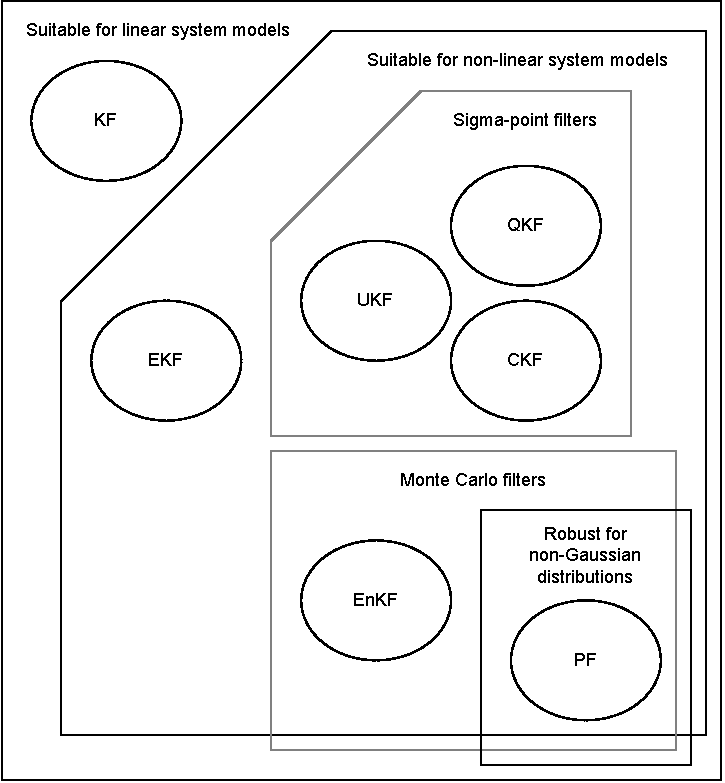
\includegraphics[width=.7\linewidth]{figures/variants-diagram.pdf}
    \caption{Diagramma di classificazione delle varianti del filtro di Kalman.}
    \label{fig:variants-diagram}
    \vspace{2\baselineskip}
\end{figure}

\section{Sviluppi recenti}

Lo studio del filtro di Kalman resta un settore vivo, a più di 60 anni dalla sua concezione. Si continuano a identificare nuovi settori di applicazione, nuove tecniche di miglioramento dell'accuratezza, della stabilità numerica e della performance computazionale. Nuove varianti, sia generiche che specializzate, si aggiungono a quelle già consolidate. Solo negli ultimi mesi si evidenziano una tecnica di ``Iteratively Saturated Kalman Filtering'' (ISKF)~\cite{yang2025}, che mira a ridurre l'impatto di eventuali misurazioni anomale, e la possibilità di affiancare una rete neurale profonda (DNN) ad un filtro classico nei cosiddetti ``AI-Aided Kalman Filters''~\cite{shlezinger2025}.

\section{Limitazioni}

Sebbene oggi assuma un ruolo fondamentale nell'ingegneria aerospaziale e in diversi altri settori, il filtro di Kalman presenta alcune limitazioni intrinseche:
\begin{itemize}
\item Per sistemi non lineari con distribuzioni non Gaussiane, non è garantita, in generale, l'ottimalità.
\item Benché la conoscenza del sistema reale sia la base dell'efficacia del filtro, questa può anche costituire un limite sulla precisione, qualora modelli sufficientemente accurati non siano disponibili.
\end{itemize}

% I suggest referencing stuff as follows: \cref{fig:random-image} or \Cref{fig:random-image}

% \begin{figure}
%     \centering
%     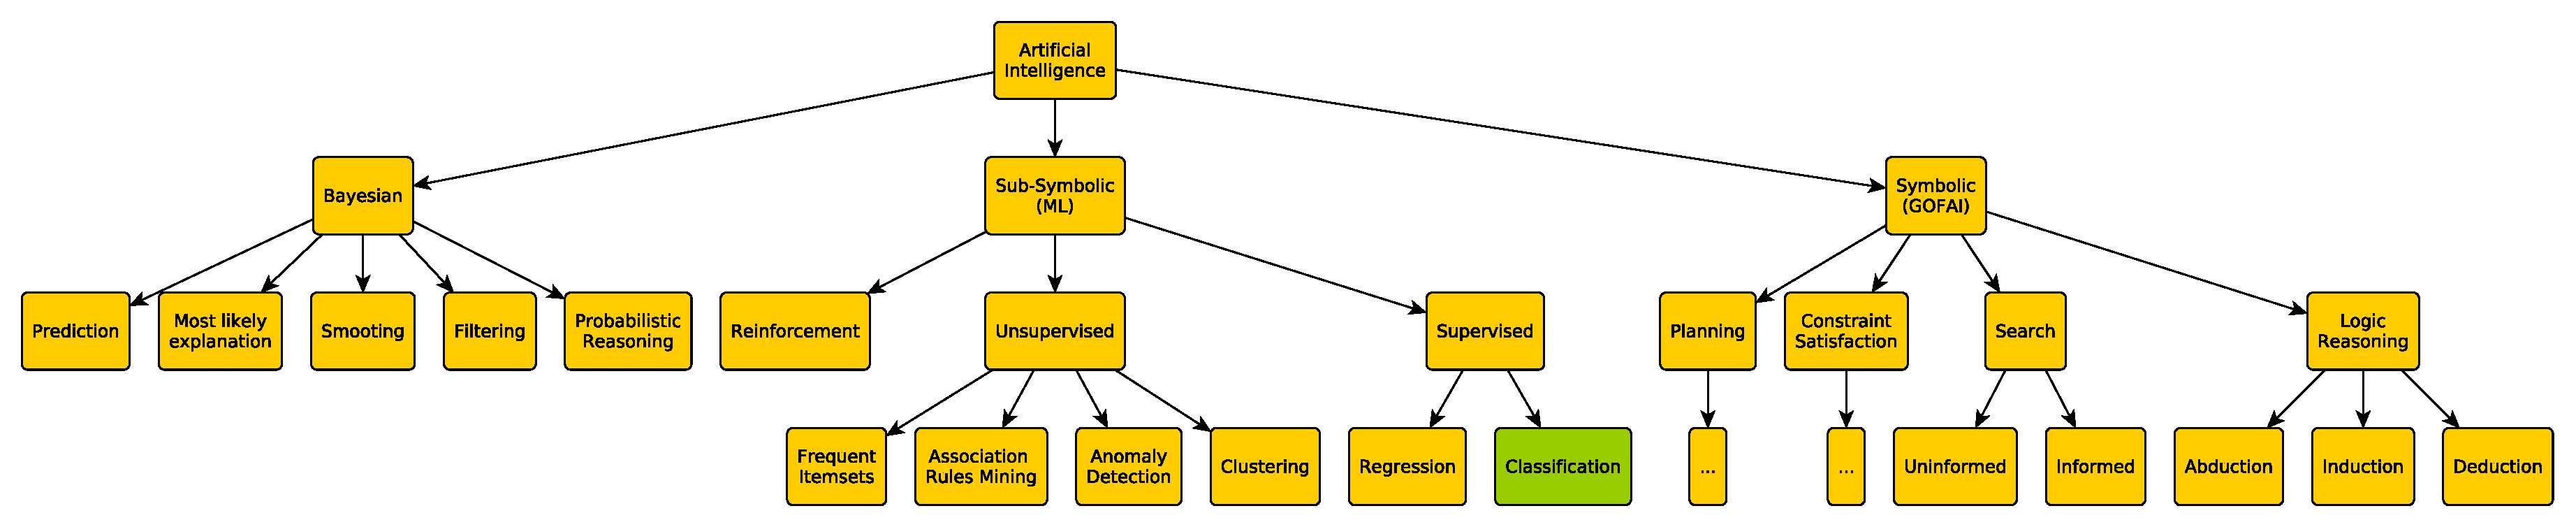
\includegraphics[width=.8\linewidth]{figures/random-image.pdf}
%     \caption{Some random image}
%     \label{fig:random-image}
% \end{figure}

% \section{Some cool topic}

\iffalse % Discarded chapter
\chapter{Evoluzione e sviluppi recenti}

Lo studio del filtro di Kalman resta un settore vivo, a più di 60 anni dalla sua concezione. Si continuano a identificare nuovi settori di applicazione, nuove tecniche di miglioramento dell'accuratezza, della stabilità numerica e della performance computazionale. Nuove varianti, sia generiche che specializzate, si aggiungono a quelle già consolidate. In questo capitolo si presenta un riassunto della storia ed evoluzione del filtro, insieme alle missioni che ne hanno dimostrato il merito, e si riportano alcuni dei progressi più recenti, fornendo un'anteprima della direzione attuale della ricerca.

\section{Dalla guerra fredda ad oggi}

Rudolf Emil Kálmán studiò i sistemi dinamici lineari a tempo discreto già nel 1954 per la sua tesi di laurea magistrale al MIT. Nel 1958, con l'intensificarsi della corsa allo spazio, il governo federale degli Stati Uniti d'America finanziò gli studi di Kálmán e del collega Richard S. Bucy per la stima e il controllo di sistemi aerospaziali. In questo contesto, a novembre dello stesso anno, nacque l'idea di riformulare il metodo di stima ottimale dell'esistente filtro di Wiener-Kolmogorov, utilizzando una rappresentazione in spazio di stato generica e spostando il problema dal dominio delle frequenze al dominio del tempo. Il filtro ottenuto rimuoveva il requisito di un modello tempo-invariante, permetteva di esprimere il modello con equazioni più semplici da ricavare e prometteva un algoritmo più adatto all'implementazione a computer.
Nel 1960, Kálmán pubblicò la descrizione del filtro a tempo discreto~\cite{10.1115/1.3662552} e nel 1961, insieme a Bucy, il filtro a tempo continuo~\cite{10.1115/1.3658902}, chiamato oggi filtro di Kalman-Bucy.
% TODO: riprendi da Schmidt

\section{Iteratively Saturated Kalman Filtering}

\section{AI-Aided Kalman Filters}
\fi

%----------------------------------------------------------------------------------------
\chapter{Modello astronomico}
%----------------------------------------------------------------------------------------

In questo capitolo si presentano le formule e i modelli teorici che governano le osservazioni di corpi celesti e il tracciamento del loro moto. Si delinea un sistema dinamico altamente non lineare, che dimostra la necessità di tecniche e algoritmi avanzati per lo studio di un caso d'uso reale.

\section{Coordinate celesti}

Le osservazioni astrometriche fanno uso di una coppia di angoli $(\alpha,\delta)$ per identificare la posizione dei corpi nella sfera celeste, o, più precisamente, per identificare la direzione orientata dall'osservatore verso la posizione apparente del corpo considerato. I due angoli sono definiti con riferimento al piano equatoriale e al punto vernale dell'epoca J2000.0 (mezzogiorno del 1° gennaio 2000, calendario gregoriano e tempo terrestre). Nella pratica si considerano assi orientati secondo il sistema ICRS, adottato dalla International Astronomical Union dal 1° gennaio 1998, spostando l'origine dal baricentro del sistema solare alla posizione dell'osservatore (osservazione topocentrica). In questo contesto, l'ascensione retta $\alpha\in[0,2\pi)$ rappresenta la rotazione attorno all'asse z, mentre la declinazione $\delta\in\left[-\frac{\pi}{2},\frac{\pi}{2}\right]$ rappresenta la distanza angolare dal piano xy. \pagebreak

Dunque, indicando con $\Delta$ la distanza apparente tra l'osservatore e il corpo al momento dell'osservazione, la posizione apparente del corpo osservato, in coordinate cartesiane topocentriche, è data da:
\begin{equation}\label{eq:radec2pos}
\begin{pmatrix} x \\ y \\ z \end{pmatrix}=R_z(\alpha)\,R_y(-\delta)\begin{pmatrix} \Delta \\ 0 \\ 0 \end{pmatrix}=\begin{pmatrix} \Delta\cos(\delta)\cos(\alpha) \\ \Delta\cos(\delta)\sin(\alpha) \\ \Delta\sin(\delta) \end{pmatrix}
\end{equation}
La conversione a coordinate baricentriche richiede semplicemente di sommare la posizione dell'osservatore rispetto al baricentro del sistema solare. \\

Si definiscono le distanze apparenti $R$ tra l'osservatore e il Sole al momento dell'osservazione e $d$ (solitamente indicata con $r$, ma da non confondersi con la distanza dal fuoco occupato dell'orbita) tra il corpo osservato e il Sole nel momento in cui la luce osservata viene riflessa sulla superficie del corpo. Si definiscono gli angoli di separazione $\theta\in[0,\pi]$, detta elongazione, tra il corpo e il Sole come appaiono all'osservatore al momento dell'osservazione e $\phi\in[0,\pi]$, detto angolo di fase, tra l'osservatore e il Sole come appaiono dal corpo nel momento in cui la luce osservata viene riflessa. Seppure si tratti di una definizione analoga, l'angolo di fase viene definito, in genere, come l'angolo tra la luce incidente e la luce riflessa verso l'osservatore, per via del suo impatto sul modello ottico descritto nella sezione \ref{sec:photometry}. \\

Si è parlato finora di quantità apparenti. Questa precisazione è necessaria per via della velocità finita della luce e ad altri fenomeni come aberrazioni, rifrazioni ed effetti relativistici. Da questo punto in poi si considereranno le quantità apparenti come coincidenti alle controparti ``reali'' (geometriche), con la consapevolezza che ciò introdurrà imprecisioni nel modello, le quali dovranno essere considerate nell'applicazione del filtro di Kalman. Queste imprecisioni sono accettabili per il tracciamento di asteroidi, ma possono diventare problematiche per oggetti più veloci.

Con questa semplificazione diventa possibile considerare il triangolo tra il corpo osservato, l'osservatore e il Sole e applicare il teorema dei seni per determinare relazioni fra gli angoli e le distanze. In particolare:
\begin{gather}
\frac{d}{\sin(\theta)}=\frac{R}{\sin(\phi)}\label{eq:sinelaw-d} \\
\frac{\Delta}{\sin(\pi-\theta-\phi)}=\frac{R}{\sin(\phi)}\Rightarrow\frac{\Delta}{\sin(\theta+\phi)}=\frac{R}{\sin(\phi)}\label{eq:sinelaw-delta}
\end{gather}

\section{Fotometria e il sistema H-G}\label{sec:photometry}

Nello studio degli asteroidi, l'intensità della luce osservata è espressa dalla magnitudine apparente e può essere utilizzata per stimare la distanza del corpo. Intuitivamente, questa quantità dipende dall'angolo di fase ($\phi\approx0$ indica un corpo perfettamente illuminato, mentre $\phi\approx1$ comporta che non venga riflessa luce verso l'osservatore), dalle distanze $d$ e $\Delta$ e da alcune caratteristiche fisiche del corpo. Tuttavia non esiste un modello macroscopico esatto.

Una delle prime applicazioni delle nozioni di fotometria allo studio degli asteroidi ha prodotto il modello H-G~\cite{bowell1989}~\cite{dymock2007}, usato tuttora quando non si dispone di informazioni sufficienti per impiegare modelli più precisi. Gli asteroidi vengono caratterizzati da due parametri: $H$, detta magnitudine assoluta, che equivale alla magnitudine apparente per $d=\Delta=1~\mathrm{AU}$ e $\phi=0$\quad e $G$, detto \textit{slope parameter}, che quantifica un picco di luminosità che spesso si verifica nella curva di fase vicino all'opposizione. Se si esprimono le distanze in unità astronomiche, la magnitudine apparente è descritta da:
\begin{gather}
V=H+5\log_{10}(d\Delta)-2.5\log_{10}(\Phi(\phi))\label{eq:hg-mag} \\
\Phi(\phi)=(1-G)\exp\left(-3.33\bigl(\tan\left(\tfrac{\phi}{2}\right)\bigr)^{0.63}\right)+G\exp\left(-1.87\bigl(\tan\left(\tfrac{\phi}{2}\right)\bigr)^{1.22}\right)
\end{gather}

\section{Orbite ellittiche}

Il moto dei pianeti, degli asteroidi e delle comete è ben approssimato da orbite ellittiche, con un fuoco occupato dal baricentro del sistema solare. \pagebreak

Tali orbite possono essere caratterizzate tramite i parametri orbitali kepleriani:
\begin{itemize}
\item il semiasse maggiore $a$;
\item l'eccentricità $e$, dove $e=0$ indica un orbita circolare, mentre $e\to 1$ descrive un'orbita progressivamente più schiacciata;
\item l'inclinazione $i\in[0,\pi]$ del piano dell'orbita, in genere espressa rispetto al piano dell'orbita della Terra, ma in questo caso espressa rispetto al piano xy del sistema di riferimento, con $i<\frac{\pi}{2}$ indicante un'orbita prograda e $i>\frac{\pi}{2}$ indicante un'orbita retrograda;
\item la longitudine del nodo ascendente $\Omega$;
\item l'argomento del periapside $\omega$.
\end{itemize}
La posizione del corpo nell'orbita è identificata dall'anomalia. Più precisamente, la distanza angolare dal periapside è detta anomalia vera e indicata con $\nu$. \\
Si definisce la distanza radiale $r$ dal fuoco occupato e l'argomento di latitudine $u=\omega+\nu$, cosicché le coordinate cartesiane del corpo siano date da:
\begin{equation}
\begin{pmatrix}x \\ y \\ z\end{pmatrix}=R_z(\Omega)R_x(i)R_z(u)\begin{pmatrix}r \\ 0 \\ 0\end{pmatrix}=\begin{pmatrix}r\bigl(\cos(\Omega)\cos(u)-\sin(\Omega)\sin(u)\cos(i)\bigr) \\ r\bigl(\sin(\Omega)\cos(u)+\cos(\Omega)\sin(u)\cos(i)\bigr) \\ r\sin(u)\sin(i)\end{pmatrix}
\end{equation}
Per studiare l'evoluzione della posizione nel tempo si introducono i concetti di anomalia media $M$ e anomalia eccentrica $E$. \\
La prima avanza linearmente nel tempo in base al moto medio $n$ e al tempo di periapside $\tau$:
\begin{equation}
M=n(t-\tau)
\end{equation}
Il moto medio è definito dal periodo dell'orbita come $n=\frac{2\pi}{T}$ ed è ricavabile dal semiasse maggiore e dal parametro gravitazionale $\mu=GM$ del corpo primario (in questo caso $G$ è la costante di gravitazione universale e $M$ è la massa del corpo primario):
\begin{equation}
n=\sqrt{\frac{\mu}{a^3}}
\end{equation}
Una volta determinata l'anomalia media, si risale all'anomalia eccentrica esprimendo gli angoli in radianti e risolvendo l'equazione di Keplero tramite metodi numerici:
\begin{equation}
M=E-e\sin(E)
\end{equation}
In questo caso si è scelto di utilizzare il metodo di Newton, ponendo $f(x)=x-e\sin(x)-M$, $f^\prime(x)=1-e\cos(x)$ e $x_0=M$. \\
Dall'anomalia eccentrica è possibile passare all'anomalia vera. Una formula numericamente stabile richiede di calcolare il valore intermedio $\beta$:
\begin{gather}
\beta=\frac{e}{1+\sqrt{1-e^2}} \\
\nu=E+2\arctan\left(\frac{\beta\sin(E)}{1-\beta\cos(E)}\right)
\end{gather}
Infine, la distanza radiale è legata all'anomalia eccentrica da:
\begin{equation}
r=a(1-e\cos(E))
\end{equation}

%----------------------------------------------------------------------------------------
\chapter{Contributo}
%----------------------------------------------------------------------------------------

TODO

\section{Approccio diretto}

Prima ancora di considerare strategie di filtraggio o di tracciamento del moto orbitale, si potrebbe pensare di risalire a una posizione direttamente dai dati osservati. In effetti, se si conoscesse la distanza del corpo $\Delta$, la si potrebbe sfruttare, insieme agli angoli $\alpha,\delta$, nella formula~\ref{eq:radec2pos}. Tuttavia, risalire a $\Delta$ dalla magnitudine visuale $V$ richiede particolare attenzione.

Idealmente, si vorrebbe sfruttare direttamente la formula~\ref{eq:hg-mag}, ma non si dispone della distanza dal Sole $d$ e dell'angolo di fase $\phi$. Una possibile soluzione prevede di risolvere in $\phi$ la seguente equazione tramite metodi numerici:
\begin{equation}
R^2\sin(\theta)\sin(\theta+\phi)-10^{0.2(V-H)}\sin^2(\phi)\sqrt{\Phi(\phi)}=0
\end{equation}
Tale equazione deriva dai seguenti passaggi:
\begin{gather*}
V=H+5\log_{10}(d\Delta)-2.5\log_{10}(\Phi(\phi)) \\
\rightarrow 0.2(V-H)+\log_{10}\left((\Phi(\phi))^{0.5}\right)=\log_{10}(d\Delta) \\
\rightarrow d\Delta=10^{0.2(V-H)}\sqrt{\Phi(\phi)}
\end{gather*}
Utilizzando le equazioni~\ref{eq:sinelaw-d} e \ref{eq:sinelaw-delta}, si trova che:
\begin{equation*}
d\Delta=\dfrac{R^2\sin(\theta)\sin(\theta+\phi)}{\sin^2(\phi)}
\end{equation*}
Sostituendo e moltiplicando entrambi i lati per $\sin^2(\phi)$ si ottiene l'espressione desiderata. Si osservi che per $\phi=0$ e $\phi=\pi$ sarebbe impossibile effettuare osservazioni valide, per cui si può assumere $\sin(\phi)\neq0$. Lo stesso vale per l'elongazione $\theta$. \\
Il vantaggio di questa specifica scrittura sta nel fatto che l'espressione ha valore positivo finito per $\phi=0$, ovvero $R^2\sin^2(\theta)$, e ha valore negativo finito per $\phi\to\pi$, ovvero $-R^2\sin^2(\theta)$, il che permette di utilizzare il metodo di Brent nell'intervallo $[0,\pi]$. \\
Una volta determinata una radice, la distanza è data da:
\begin{equation}
\Delta=\dfrac{R\sin(\theta+\phi)}{\sin(\phi)}
\end{equation}
Si osservi che in generale può esistere più di una radice, specie se l'elongazione $\theta$ è piccola; tuttavia questo non si verifica nei dataset considerati. \\
In ogni caso, questo processo è estremamente sensibile all'errore sui dati iniziali e la magnitudine risulta essere una misura piuttosto imprecisa. Tutto ciò evidenzia ulteriormente la necessità di strategie più sofisticate. \\
Questo approccio iniziale resta comunque un utile punto di riferimento e verrà utilizzato per quantificare l'efficacia del filtro di Kalman in questo contesto.

Per il calcolo di $R$ e $\theta$ si può sfruttare un servizio di effemeridi. In questo caso si è utilizzato il servizio JPL, sia attraverso la funzione \lstinline{astropy.coordinates.solar_system.get_body_barycentric}, che dalla piattaforma web \url{https://ssd.jpl.nasa.gov/horizons/app.html}. \\
Indicando con $\hat{R}$ il versore dall'osservatore verso il sole e con $\hat{\Delta}$ il versore dall'osservatore verso il corpo, l'elongazione è data da:
\begin{equation}
\theta=\arccos\left(\hat{\Delta}\cdot\hat{R}\right)
\end{equation}
Con $\hat{\Delta}$ dato da:
\begin{equation}
\hat{\Delta}=\begin{pmatrix}
\cos(\delta)\cos(\alpha) \\
\cos(\delta)\sin(\alpha) \\
\sin(\delta)
\end{pmatrix}
\end{equation} \\

% TODO: mostrare il codice che implementa?

Si procede ora con l'impostazione del problema sotto forma di sistema dinamico, come richiesto dal filtro di Kalman.

\section{Sfide sul tracciamento di angoli}

Per via della natura del problema, si vuole memorizzare quantità angolari sia nel vettore di stato che nel vettore di misurazione. Tuttavia, fare ciò senza dovuti accorgimenti introdurrebbe forti discontinuità nelle equazioni che descrivono il sistema. Si noti, ad esempio, che all'avanzare dell'anomalia, questa passa da $\nu\approx2\pi$ a $\nu\approx0$. In aggiunta, una stima $\hat{\nu}\approx2\pi$ affiancata ad una misurazione $\nu\approx0$ è in realtà da considerarsi valida, ma dal punto di vista del filtro apparirebbe come una grossa discrepanza.

Per affrontare questo problema, si decide di non memorizzare direttamente gli angoli, ma bensì di rappresentarli nelle loro componenti sulla circonferenza unitaria, ossia la coppia $\bigl(cos(\cdot),sin(\cdot)\bigr)$. Questo approccio è analogo alla rappresentazione di rotazioni in tre dimensioni attraverso l'uso di quaternioni e permette di rimuovere le discontinuità di cui si è parlato.

In figura~\ref{fig:angle-method-comparison} si mostra l'efficacia di questa soluzione applicata alla simulazione di un corpo in moto circolare uniforme.

Tuttavia restano delle limitazioni, dovute al fatto che questa trasformazione è pressoché lineare solo per piccoli errori sugli angoli. Ne segue, ad esempio, che la media fra due coppie di componenti possa non corrispondere esattamente alla media dei due rispettivi angoli, oppure possa non risiedere precisamente sulla circonferenza unitaria.

\begin{figure}
    \centering
    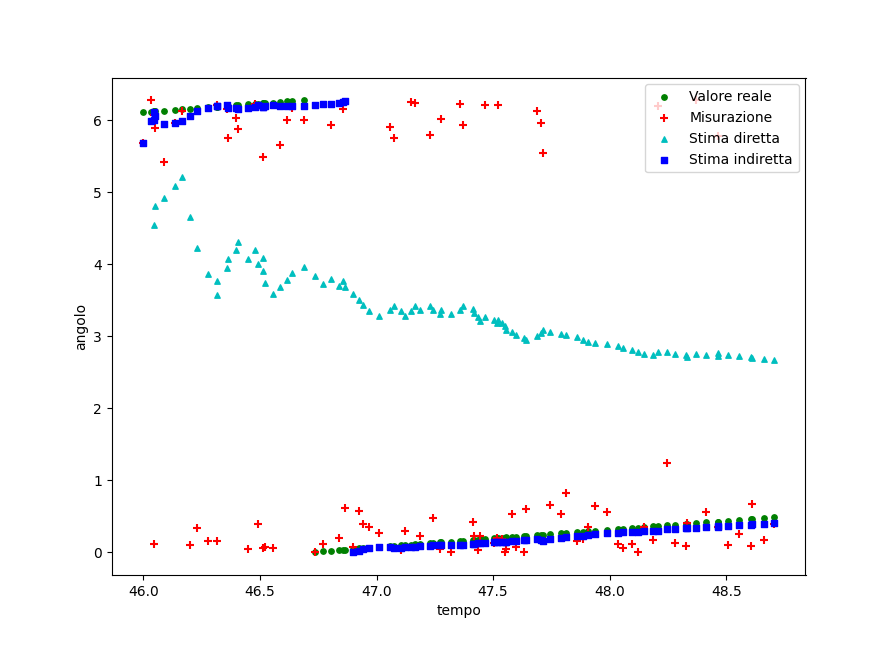
\includegraphics[width=\linewidth]{figures/angle-method-comparison.png}
    \caption{Confronto dei metodi per la stima di angoli.}
    \label{fig:angle-method-comparison}
    \vspace{2\baselineskip}
\end{figure}

\section{Scelta dei vettori di stato e di misurazione}

\begin{equation}
z=\begin{pmatrix}
\cos(\alpha) \\
\sin(\alpha) \\
\cos(\delta) \\
\sin(\delta) \\
V
\end{pmatrix}
\end{equation}
\begin{equation}
x=\begin{pmatrix}
\cos(M) \\
\sin(M) \\
a \\
e \\
\cos(i) \\
\sin(i) \\
\cos(\Omega) \\
\sin(\Omega) \\
\cos(\omega) \\
\sin(\omega) \\
n \\
H \\
G
\end{pmatrix}
\end{equation}

TODO

\section{Equazioni del sistema}

TODO

\section{Matrici di covarianza}

TODO

\section{Simulazione}

TODO

\section{Applicazione a dati reali}

Il Minor Planet Center raccoglie dati su osservazioni ottiche astrometriche di corpi minori, comete e satelliti naturali, effettuate da osservatori in tutto il mondo. I dati sono forniti senza alcun tipo di correzione, come specificato nelle linee guida (\url{https://minorplanetcenter.net/iau/info/Astrometry.html#corrs}).

Moduli Python esistenti come \lstinline{astroquery} consentono di richiedere automaticamente le osservazioni; tuttavia si possono scaricare archivi più completi direttamente dalla piattaforma web \url{https://www.minorplanetcenter.net/db_search}.

Questi archivi sono file di testo in classico stile Fortran a 80 colonne e seguono il formato descritto alla pagina \url{https://www.minorplanetcenter.net/iau/info/OpticalObs.html}. In particolare, contengono le seguenti informazioni di nostro interesse:
\begin{itemize}
% \item il metodo di osservazione utilizzato (fotografico, CCD, CMOS, ...)
\item l'ascensione retta, espressa come angolo orario, minuti e secondi
\item la declinazione, espressa in gradi, minuti e secondi
\item la magnitudine osservata
\item la banda utilizzata, ossia un'indicazione della fascia di frequenze elettromagnetiche considerate
\item il codice dell'osservatorio
\end{itemize}
Il file \lstinline{parse.py} si occupa dell'interpretazione dei dati e della trasformazione in oggetti \lstinline{MinorPlanetObservation}. Questo passaggio richiede la conversione degli angoli in radianti e della magnitudine osservata in magnitudine visuale. In effetti, i modelli fotometrici si basano sulla magnitudine relativa alla luce visibile, per cui può essere necessario utilizzare la tabella di conversione fornita alla pagina \url{https://www.minorplanetcenter.net/iau/info/BandConversion.txt}. \\
Infine, il codice dell'osservatorio viene confrontato con la lista alla pagina \url{https://www.minorplanetcenter.net/iau/lists/ObsCodes.html}, per risalire alle coordinate geodetiche dell'osservatore.

\iffalse % Template chapter
\chapter{Contribution}

You may also put some code snippet (which is NOT float by default), eg: \cref{lst:random-code}.

\lstinputlisting[float,language=Java,label={lst:random-code}]{listings/HelloWorld.java}

\section{Fancy formulas here}
\fi

%----------------------------------------------------------------------------------------
% BIBLIOGRAPHY
%----------------------------------------------------------------------------------------

\backmatter

% \nocite{*} % Remove this as soon as you have the first citation

% \bibliographystyle{alpha}
\bibliographystyle{ieeetr}
\bibliography{bibliography}

\begin{acknowledgements} % this is optional
Optional. Max 1 page.
\end{acknowledgements}

\end{document}
